\documentclass[12pt]{article}

\usepackage{fullpage}
\usepackage{multicol,multirow}
\usepackage{tabularx}
\usepackage{ulem}
\usepackage{graphicx}%Вставка картинок правильная
\usepackage{float}%"Плавающие" картинки
\usepackage{wrapfig}%Обтекание фигур (таблиц, картинок и прочего)
\usepackage[utf8]{inputenc}
\usepackage[russian]{babel}

% Оригиналный шаблон: http://k806.ru/dalabs/da-report-template-2012.tex

\begin{document}

\section*{Лабораторная работа №\,2 по курсу дискрeтного анализа: словарь}

Выполнил студент группы 08-207 МАИ \textit{Дегтярев Денис Андреевич}.

\subsection*{Условие}

Для реализации словаря из предыдущей лабораторной работы, необходимо провести
исследование скорости выполнения и потребления оперативной памяти. В случае вы-
явления ошибок или явных недочётов, требуется их исправить.

\subsection*{Дневник выполнения работы}

Для проверки скорости работы функций использовал gprof, утечки памяти находил с помощью valgrind. 
Две эти утилиты запускал на 2 тестах разных размеров: 5(только Insert) и $10^4$(все операции). 
gprof на двух тестах сразу же показал высокую скорость(время выполнения любой функции было 
принебрежимо мало), поэтому не оптимизировал код на скорость после отправки кода. Для качественной
проверки на valgrind отключил оптимизаторы в начале main. При отправке в первый раз
valgrind ругается на неизвестный key внутри класса TNode. В деструкторе я совершаю delete[] key, 
а key неицилизирован, пишет valgrind... Понял, что его нужно удалять, тк это new char[], но удалять
не дают, тк не знают, что это. Решил данную проблему инициализировав данный TNode* как nullptr 
и при каждом добавлении nullptr приравнивался к new TNode, те мы не создавали безполезные TNode.  

P.S. код оптимизировал только после "OK" отправки, тк о 3 лабе узнал замного позже отправки...

\subsection*{Первый запуск программы с помощью valgrind}

\begin{figure*}[ht!]
    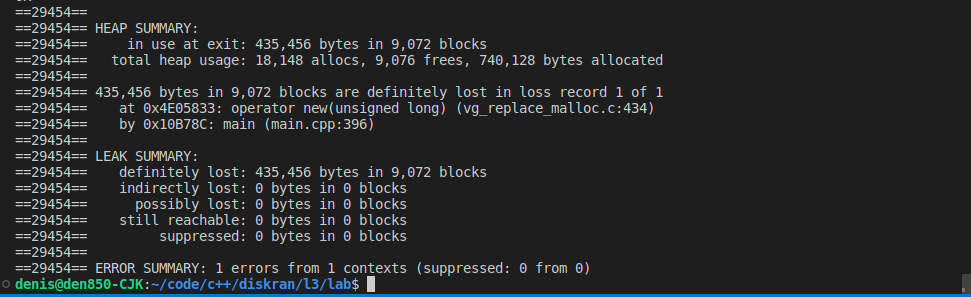
\includegraphics[width=.99\textwidth]{v3.png}
\end{figure*}

\subsection*{Итоговый запуск программы с помощью valgrind}

\begin{figure*}[ht!]
    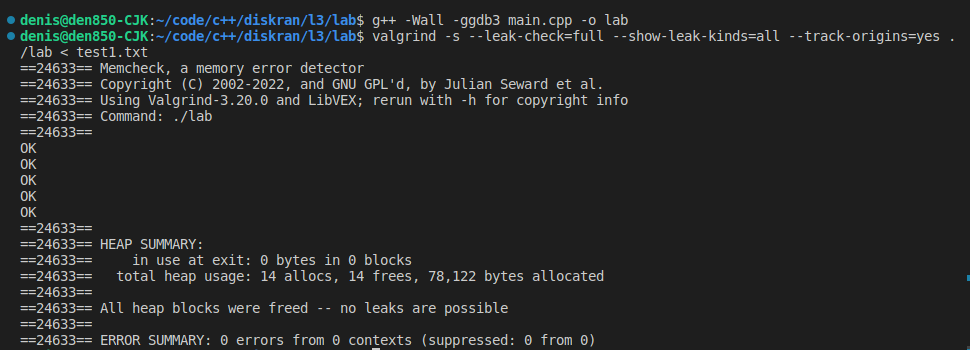
\includegraphics[width=.99\textwidth]{v1.png}
\end{figure*}

\begin{figure*}[ht!]
    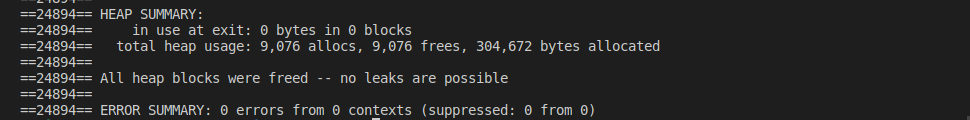
\includegraphics[width=.99\textwidth]{v2.png}
\end{figure*}

\subsection*{Итоговый запуск программы с помощью gprof}

\begin{figure*}[ht!]
    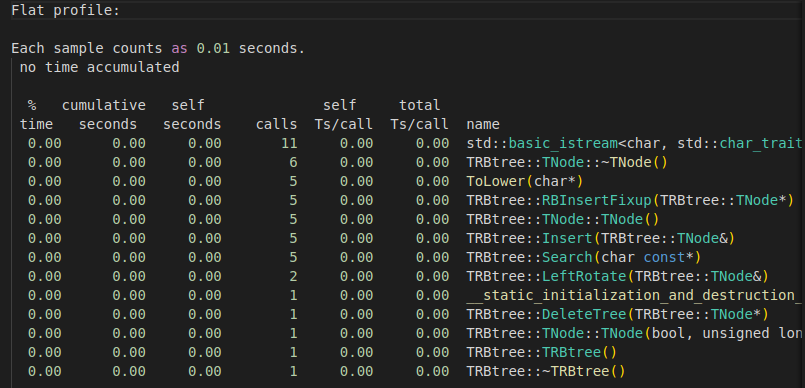
\includegraphics[width=.99\textwidth]{g1.png}
\end{figure*}

\begin{figure*}[ht!]
    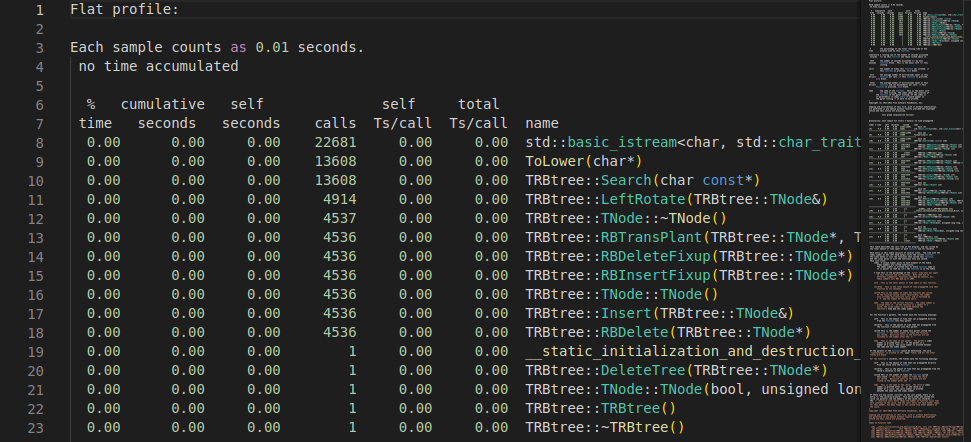
\includegraphics[width=.99\textwidth]{g2.png}
\end{figure*}

\subsection*{Выводы}

Существуют множество утилит, которые помогают нам оптимизировать код программы и найти различные 
утечки в ходе выполнения. Для проверки моего кода на надежность и скорость помогли gprof и valgrind. 
Эти мощные утилиты не только сказали мне, что у меня где-то есть проблемы, но и указали где(
удобно, когда тебе пишут в какой  строчке у тебя ошибка и почему или когда ты знаешь в какой функции беда...). 
Данные инструменты очень полезны и ими нельзя принебреать при работе  с  указателями.

\end{document}
